Wie zuvor gezeigt wurde, erreicht der Grovers Suchalgorithmus eine quadratische Beschleunigung im Vergleich zu klassischen Suchalgorithmen in unstrukturierten Datenmengen. 
Gerade im Hinblick auf $\mathbf{NP}$-vollständige Probleme stellt sich jedoch die Frage, ob eine noch größere Beschleunigung erreicht werden kann. Der Idealfall wäre eine exponentielle Beschleunigung der Suche. 
Diese Beschleunigung ist jedoch mit dem Grovers-Algorithmus nicht erreichbar. 
Es ist bewiesen, dass Grovers optimal ist \cite[S. 161-166]{Ho17}. 
Diese Limitierung ist relevant, wenn die Anwendungsmöglichkeiten von Grover betrachtet werden.
\subsection{klassische Datenbanken}
Grundsätzlich kann der Grover-Algorithmus eingesetzt werden, um klassische Datenbanken zu durchsuchen. 
Dazu wird allerdings ein aufwendiges Adressierungssystem benötigt, um die Verbindung zwischen klassischer Datenbank und Quantenhardware herzustellen. 
Ob dies zukünftig ein praktikabler Einsatzort für Quantensuchen wird, ist abhängig von der Entwicklung der verfügbaren Quantenhardware und deren Preisentwicklung.
\subsection{NP-vollständige Probleme}
Weiterhin lässt sich der Grovers-Algorithmus grundsätzlich für jedes Problem aus $\mathbf{NP}$ anwenden. 
So kann beispielsweise für das Traveling Salesperson Problem mithilfe der G-BBHT-Suche aus Kapitel \ref{gbbht} in $\mathbf{O(\sqrt{N})}$ eine Rundreise gefunden werden, die kürzer ist als eine gegebene Rundreise $\mathbf{k}$. 
Mit der Suche nach dem Minimum aus Kapitel \ref{minimum} kann sogar die kürzeste Rundreise aus $\mathbf{N}$ gefunden werden.

\begin{figure}
    \centering
	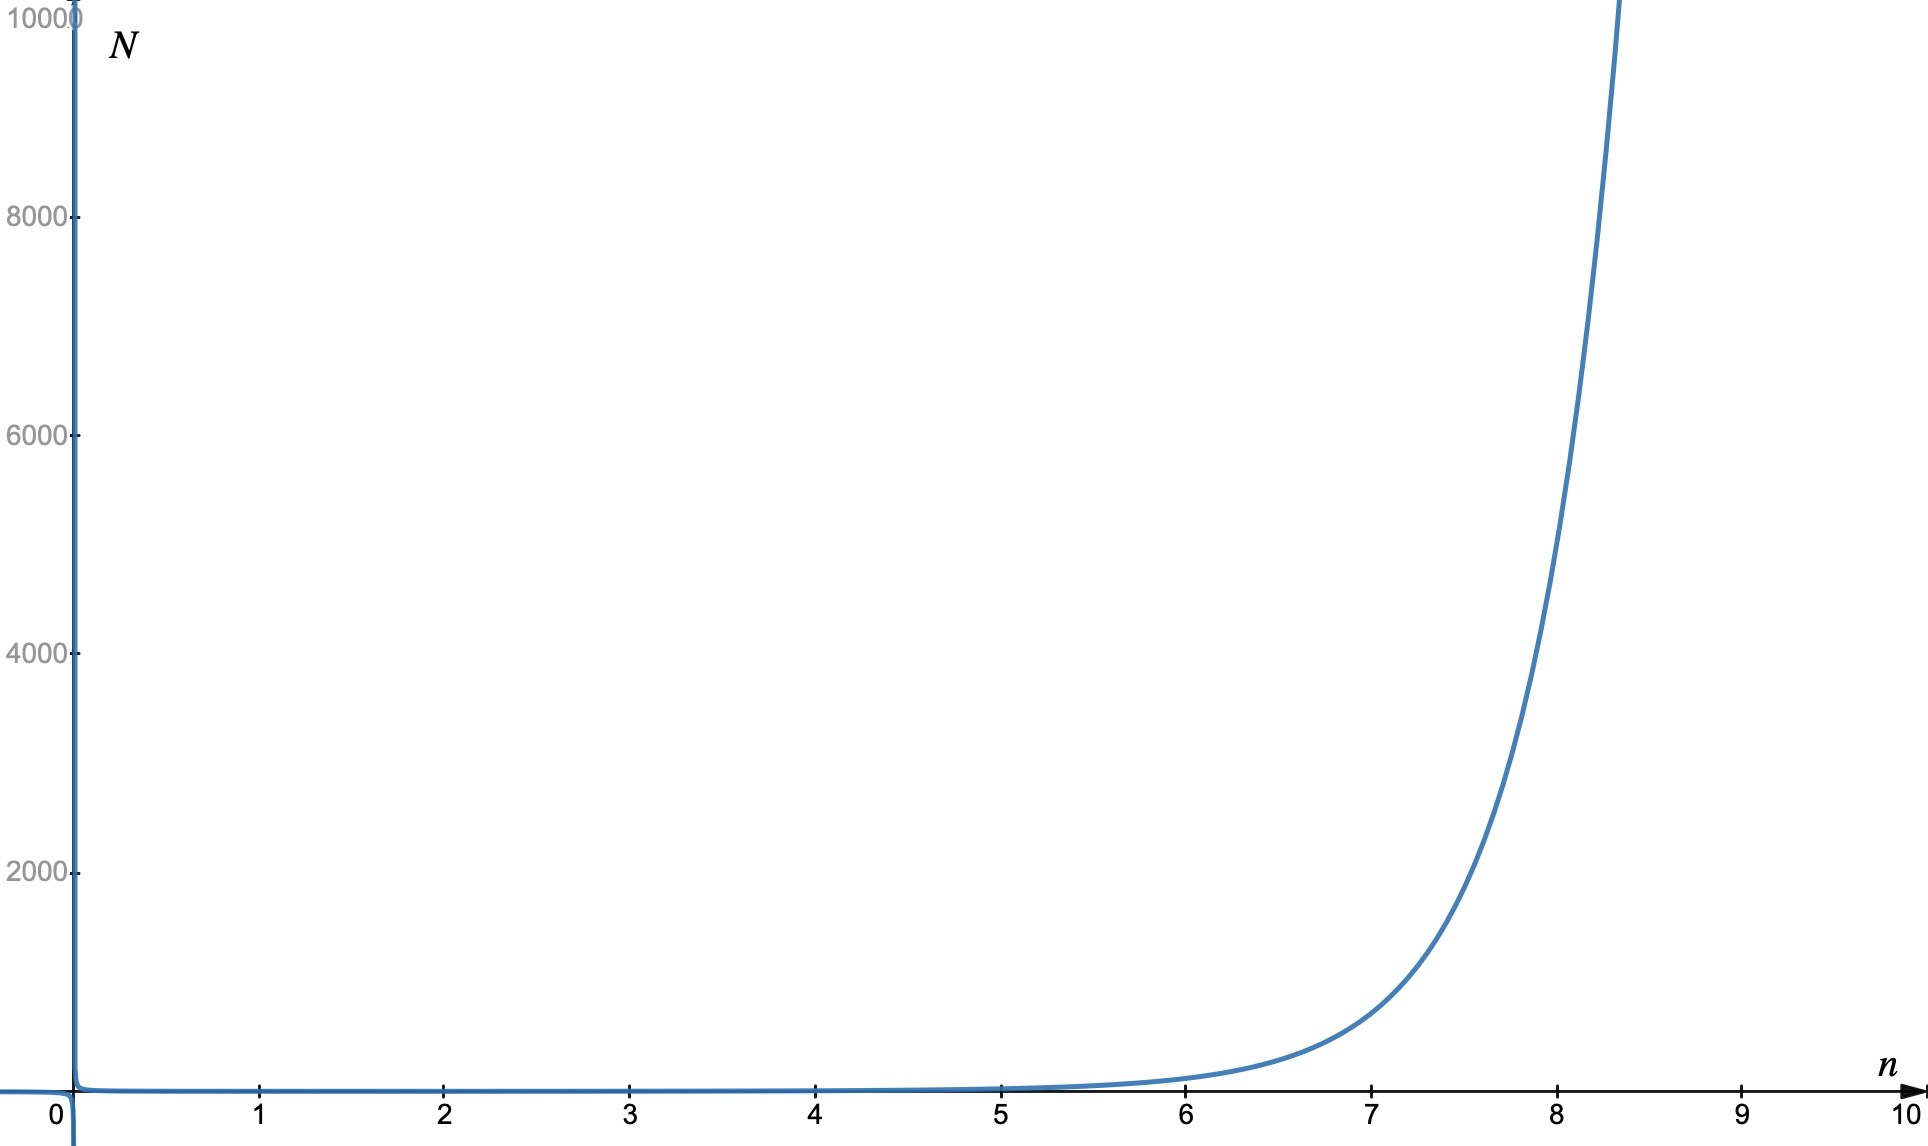
\includegraphics[width=0.7\textwidth]{figures/tsp.jpg}

    \caption{Exponentielles Wachstum der möglichen Rundreisen mit steigender Anzahl der Städte\\Quelle: Eigene Darstellung}

	\label{fig:tsp}
\end{figure}

In $\mathbf{N}$ liegt jedoch das limitierende Problem. Sollen beispielsweise $\mathbf{n}$ Städte besucht werden, so ergeben sich $\mathbf{N=(n-1)!}$ mögliche Rundreisen. 
\Cref{fig:tsp} zeigt, wie $\mathbf{N}$ im Verhältnis zu der Anzahl der Städte exponentiell wächst und somit verheerend groß wird. 
Die quadratische Beschleunigung durch den Grovers Algorithmus ist nicht ausreichend, um dieses Problem mit polynomialen Aufwand lösen zu können. 
Dazu wäre eine exponentielle Beschleunigung der Suche notwendig, dann könnte das Problem mit $\mathbf{\theta (n * \log n)}$ gelöst werden können. 
Da jedoch bewiesen ist, dass Grovers Algorithmus optimal ist, ist dies unmöglich.